\section{Problem Statement}
\label{sec:problemStatement}

\emph{\color{blue} TODO: referansene må oppdateres.}

ACO has several advantages for the VRP, such as natural parallelism and continuous positive feedback, which allows good solutions to be identified fast. However, ACO also has a few drawbacks including the weakness of getting stuck at a local optima. We will investigate the possibility of overcoming this drawback and to enhance the optimization process, by improving ACO, and including features from other swarm inspired methods. As stated in Section \vref{sec:relatedWork}, we only found one attempt to combine different methods from swarm intelligence.% is to add a notion of the global best solution found to ACO and BCO. 

We did not manage to find any previous research that used graph databases in combination with the vehicle routing problem and swarm intelligence. As mentioned in \vref{subsubsec:neo4j}, does the graph database Neo4j \citep{website:neo4j} have several advantageous features for managing graphs, and we will therefore determine potential advantages and disadvantages of using Neo4j in our implementation and in the optimization process, giving us research question \vref{itm:3a}.

The current solution of AtB consist of an experience based route network, and therefore not properly, computationally optimized concerning the travel demand and travel time. When a route network is not properly optimized, it can lead to a large number of transfers for passengers when they are traveling from their origin to their destination, resulting in a long total travel time. A good route network will ensure that routes having the most traveling demands are satisfied with short paths and few vehicle transfers, making travel demand a key variable for the algorithm. AtB\citep{website:atb} does not possess accurate data about the travel demand, and detailed investigations into measuring and predicting travel demand is a complex research problem, and beyond the scope of this thesis. 

Demand values and travel times are all provided for Mandl's benchmark problem\citep{mandl79}, and will in this thesis be used as the input data. Illustrated in \vref{fig:MandlNetwork_problemstatement}, includes the data a small and dense network with 15 nodes and 21 edges. For the urban transit network design problem (UTNDP), Mandl's network seems to be the only benchmark instance used and acknowledged by researchers\citep{fan09},\citep{kechagiopoulos14},\citep{nikolic14}. The algorithms are compared with regard to the percentage of total transfer demands satisfied directly ($d_0$), with one transfer ($d_1$), two transfers ($d_2$), or with more than two transfers or not satisfied at all ($d_{unsat}$). The algorithms are also compared regarding average in-vehicle travel time ($ATT$). The experiments are conducted on route set designs with four, six, seven and eight routes.

%Christoph Mandl\citep{mandl79} developed a heuristic algorithm for the UTRP, and the method was applied and based on a real network in Switzerland, the Swiss transit network\citep{mandl80}. 
 %The total demand for the network is 15,570 trips per day, which is a relatively high demand for a small network.
\begin{figure}[H]
\begin{center}
  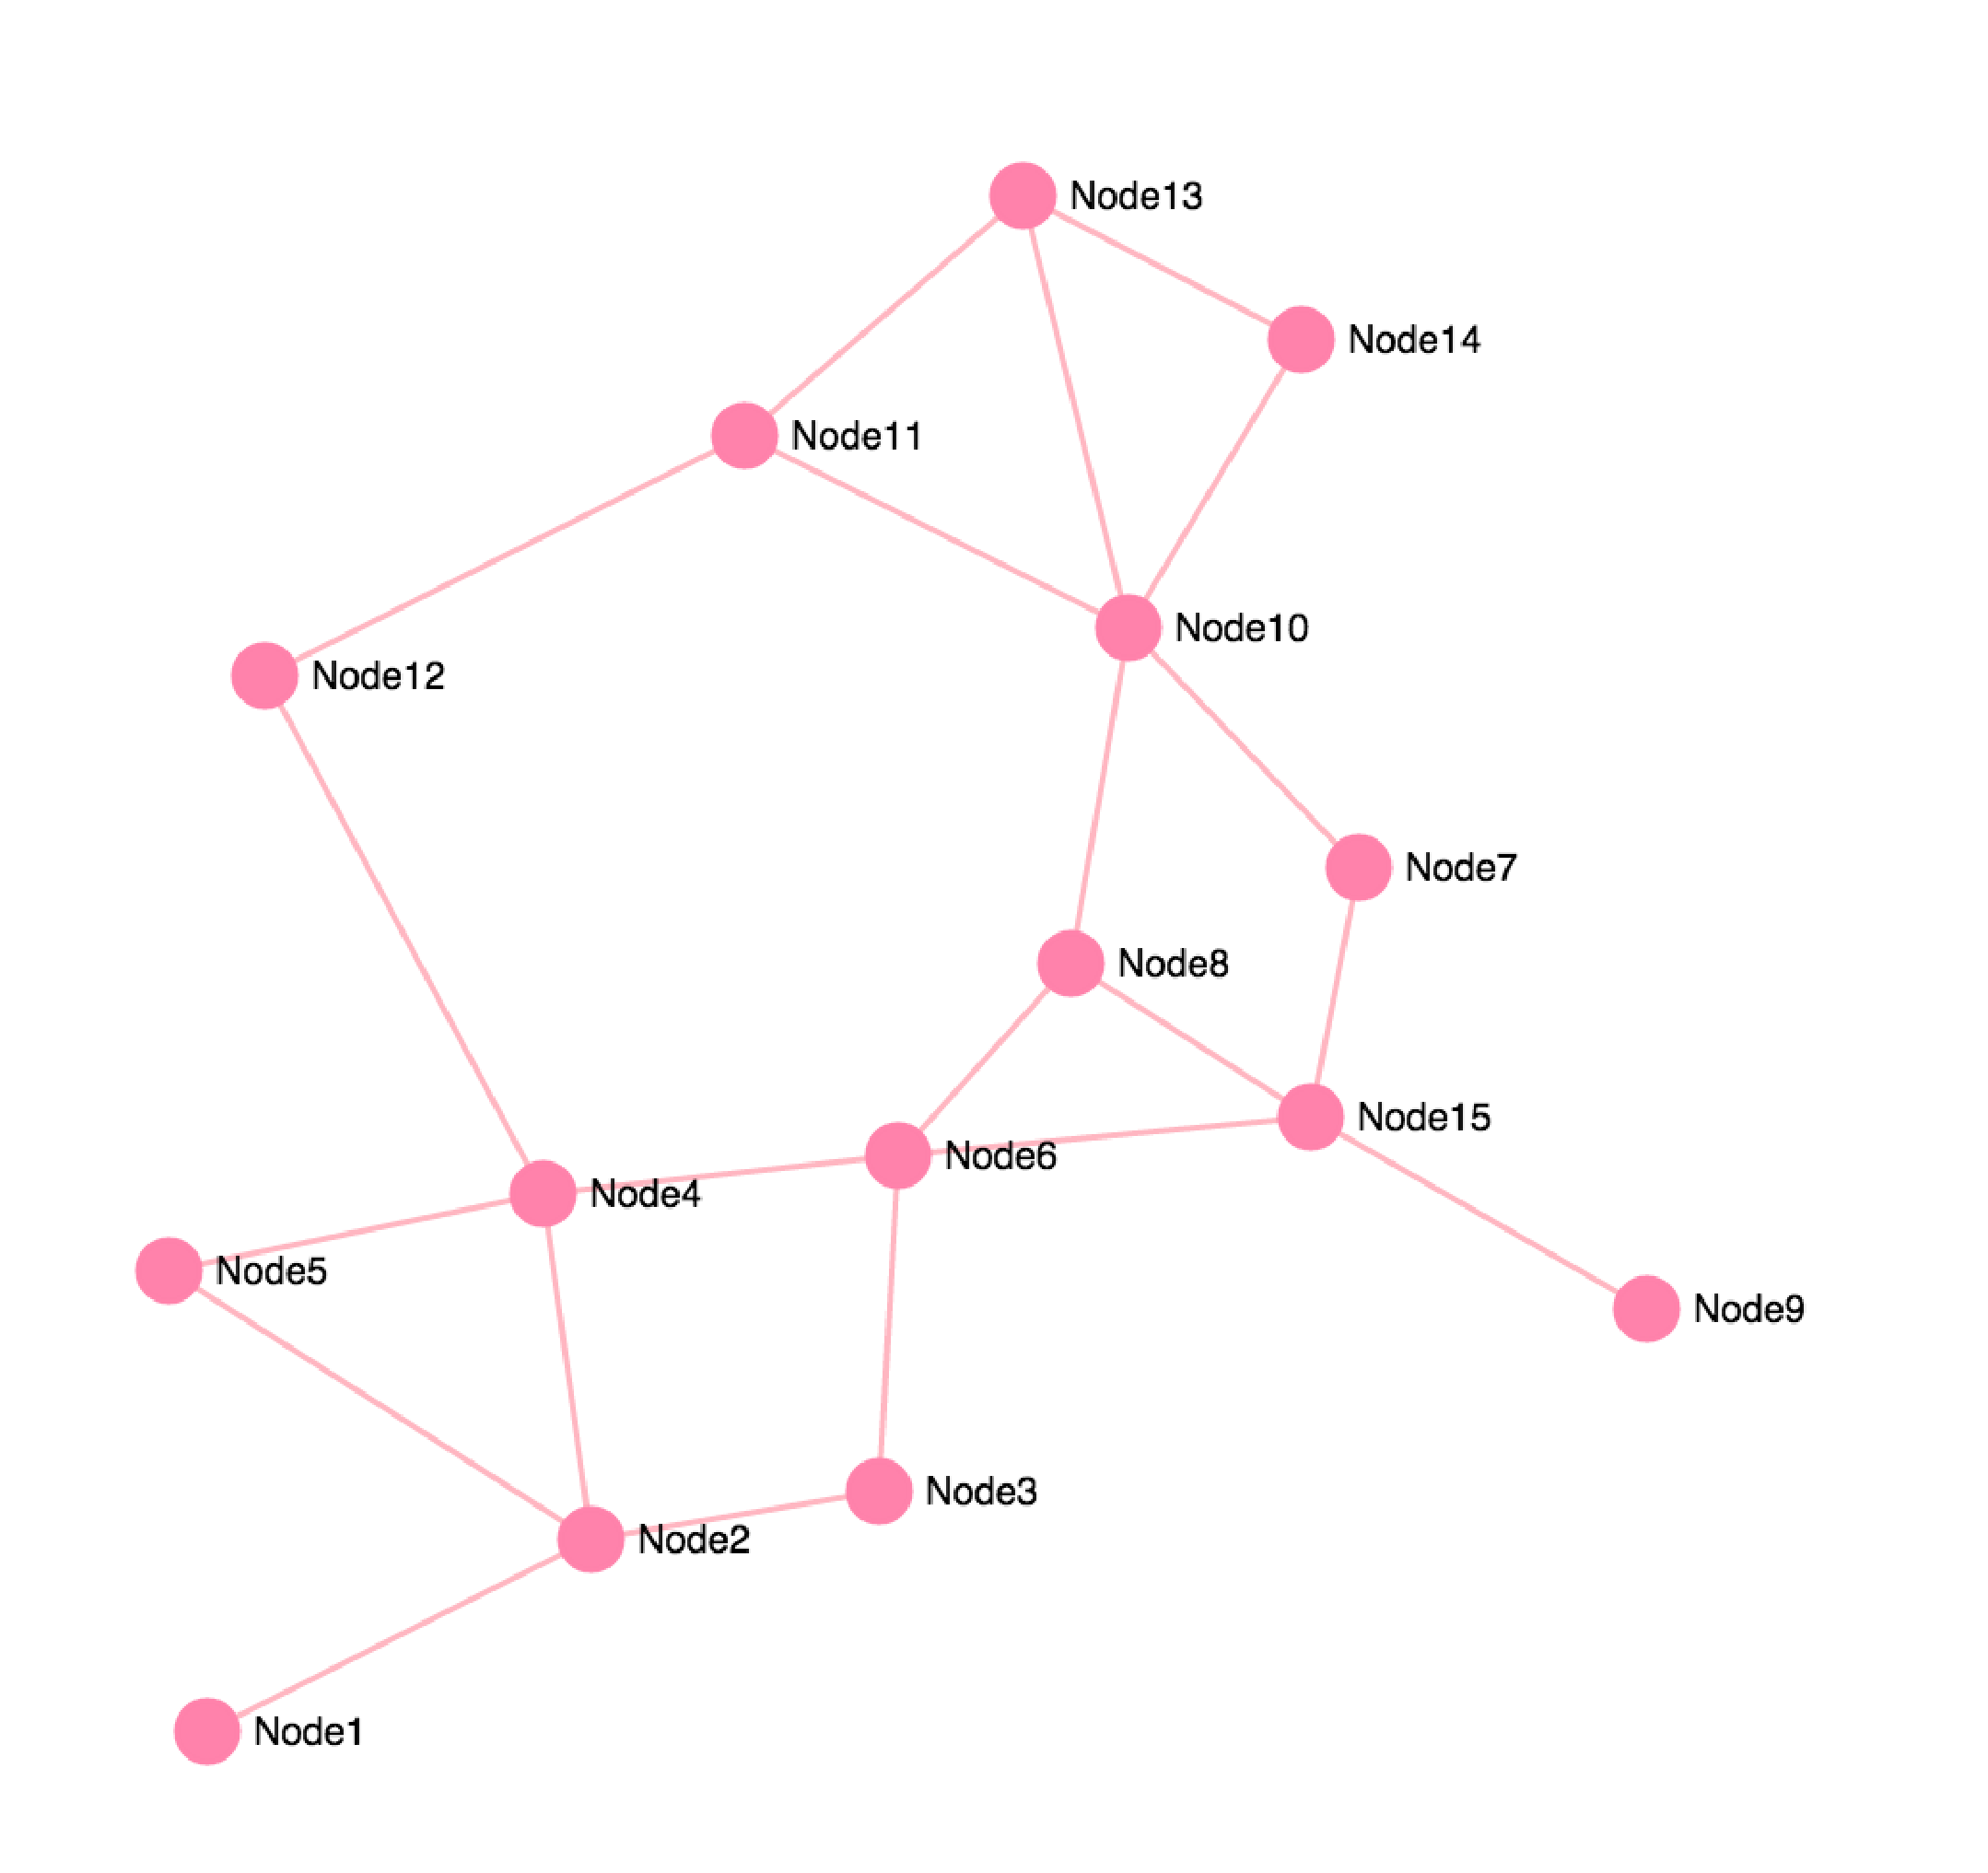
\includegraphics[width=4in]{assets/mandlnetwork_crop.png}
  \end{center}
  \caption{Illustration of Mandl's transit network as a graph}
  \label{fig:MandlNetwork_problemstatement} 
   %The transit network including the 15 nodes and 21 edges. The graph is undirected. \emph{\color{blue} TODO: Assumptions that it is undirected} Coordinates are correct based on the MandlCoordinates.txt file from \citep{mumford13}
\end{figure}

%\begin{itemize}
%\item The percentage of demand satisfied without any transfers, which should be as high as possible.
%\item The percentage of total transfer demands where the number of transfers are 1, which should be as low as possible.
%\item The percentage of total transfer demands where the number of transfers are 2, which should be as low as possible.
%\item The percentage of unsatisfied travelers, which should be equal to zero. An unsatisfied traveler is described as a traveler with 3 or more transfers.
%\item The average travel time in minutes per transit user, which should be as low as possible. %The travel times incorporates a transfer penalty, which is sat to be 5 minutes per transfer for comparison reasons. 
%\end{itemize}

For the reasons stated above, we will in this thesis focus on the UTRP, creating effective urban transit routes, with an ACO algorithm inspired by both BCO and PSO, and compare the results with the performance criteria used in similar research. This will help us establish Research Question \vref{itm:2a}, which is concerned about whether or not it is efficient to combine attributes from different swarm intelligence methods in order to improve the computational results.

Our goal with our implementation is that it further can be used to optimize AtBs transit network in order to increase the number of public transportation passengers. Research Question \vref{itm:2c} is concerned about whether or not it is possible to apply our algorithm to optimize bus routes in urban cities. This question cannot be fully answered until it is applied to an urban city, but we will strive to create a method that is easily adaptable with the concerns of public transportation in cities in mind. The implementation will be easily changed with new demand values, and tested on other larger networks.


